% Composition 1 — Cord
% El Gólem, 2026-05-23
%
% The quipu metaphor rendered as Kandinsky composition. A horizontal
% primary cord with subsidiary cords descending, each cord wearing
% knots of different colors. The knot at the convergence is the
% diamond's join, the moment the cord becomes legible as one object.
\documentclass[tikz,border=4mm]{standalone}
\usepackage[T1]{fontenc}
\usepackage{xcolor}
\definecolor{kr}{HTML}{c83727}   % Kandinsky red
\definecolor{ky}{HTML}{e8b73a}   % yellow
\definecolor{kb}{HTML}{2b62a8}   % blue
\definecolor{kg}{HTML}{2a7a4d}   % deep green
\definecolor{kw}{HTML}{f4ead8}   % wash
\definecolor{ki}{HTML}{1a1a1a}   % ink
\begin{document}
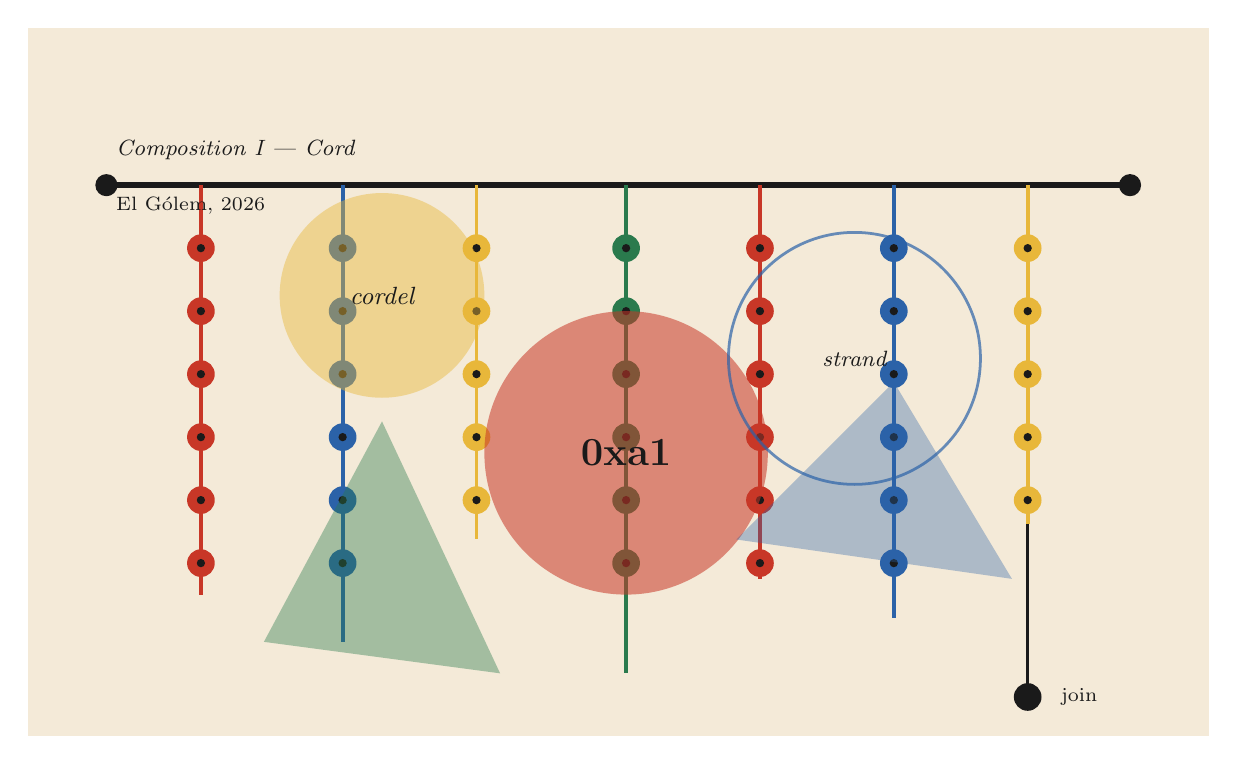
\begin{tikzpicture}[x=1cm,y=1cm]
  \fill[kw] (-1,-7) rectangle (14,2);

  % Primary horizontal cord (the central thread the whole composition hangs from)
  \draw[ki,line width=2.4pt] (0,0) -- (13,0);
  \fill[ki] (0,0) circle (4pt);
  \fill[ki] (13,0) circle (4pt);

  % Subsidiary cords (strands) descending — each one a Kandinsky color
  \foreach \x/\c/\h in {1.2/kr/5.2, 3.0/kb/5.8, 4.7/ky/4.5, 6.6/kg/6.2, 8.3/kr/5.0, 10.0/kb/5.5, 11.7/ky/4.3} {
    \draw[\c,line width=1.4pt] (\x,0) -- (\x,-\h);
  }

  % Knots along each strand — colored dots at regular intervals
  \foreach \x/\c/\h in {1.2/kr/5.2, 3.0/kb/5.8, 4.7/ky/4.5, 6.6/kg/6.2, 8.3/kr/5.0, 10.0/kb/5.5, 11.7/ky/4.3} {
    \foreach \y in {-0.8,-1.6,-2.4,-3.2,-4.0,-4.8} {
      \ifdim \y pt > -\h pt
        \fill[\c] (\x,\y) circle (5pt);
        \fill[ki] (\x,\y) circle (1.5pt);
      \fi
    }
  }

  % Large floating geometric overlays (Kandinsky-style abstraction)
  \fill[kr,opacity=0.55] (6.6,-3.4) circle (1.8);
  \fill[ky,opacity=0.45] (3.5,-1.4) circle (1.3);
  \draw[kb,line width=1.0pt,opacity=0.7] (9.5,-2.2) circle (1.6);
  \fill[kg,opacity=0.4] (2,-5.8) -- (5,-6.2) -- (3.5,-3.0) -- cycle;
  \fill[kb,opacity=0.35] (8,-4.5) -- (11.5,-5.0) -- (10,-2.5) -- cycle;

  % Floating glyphs / signifiers
  \node[ki,font=\Large\bfseries] at (6.6,-3.4) {\textbf{0xa1}};
  \node[ki,font=\itshape\small] at (3.5,-1.4) {cordel};
  \node[ki,font=\itshape\footnotesize] at (9.5,-2.2) {strand};

  % A long descending line from the rightmost knot — the join
  \draw[ki,line width=1.0pt] (11.7,-4.3) -- (11.7,-6.5);
  \fill[ki] (11.7,-6.5) circle (5pt);
  \node[ki,font=\scriptsize,anchor=west] at (12.0,-6.5) {join};

  % Annotation at top-left
  \node[ki,font=\itshape\footnotesize,anchor=south west] at (0,0.2) {Composition I --- Cord};
  \node[ki,font=\scriptsize,anchor=south west] at (0,-0.5) {El G\'olem, 2026};
\end{tikzpicture}
\end{document}
